\documentclass[pdflatex,compress,mathserif]{beamer}

%\usetheme[dark,framenumber,totalframenumber]{ElektroITK}
\usetheme[darktitle,framenumber,totalframenumber]{ElektroITK}
\usepackage[utf8]{inputenc}
\usepackage[T1]{fontenc}
\usepackage{lmodern}
\usepackage{amsmath}
\usepackage{amsfonts}
\usepackage{amssymb}
\usepackage{graphicx}
\usepackage{multicol}
\usepackage{lipsum}
\setbeamertemplate{caption}[numbered]\setbeamertemplate{caption}[numbered]
\newcommand*{\Scale}[2][4]{\scalebox{#1}{$#2$}}%

\title{Signals and Systems}
\subtitle{The Fourier Transform}

\author{Mifta Nur Farid}

\begin{document}

\maketitle

\begin{frame}
	\frametitle{From Discrete Fourier Series to Fourier Transform:}
	\begin{itemize}
		\item Let $ x[n] $ be a nonperiodic sequence of finite duration. That is, for some positive integer $ N_1 $,
	
		\begin{equation*}
			x[n] = 0~~~~|n|>N_1
		\end{equation*}
	
		Such a sequence is shown in Fig. \ref{fig:img01}.
		
		\begin{figure}
			\centering
			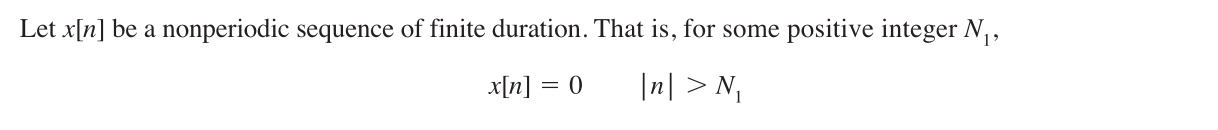
\includegraphics[width=\linewidth]{img/img01}
			\caption{Nonperiodic finite sequence $ x[n] $}
			\label{fig:img01}
		\end{figure}
		
	\end{itemize}
\end{frame}

\begin{frame}{From Discrete Fourier Series to Fourier Transform:}
	\begin{itemize}
		\item Let $ x{N_0}[n] $ be a periodic sequence formed by repeating $ x[n] $ with fundamental period $ N_0 $ as shown in Fig. \ref{fig:img02}.
		
		\begin{figure}
			\centering
			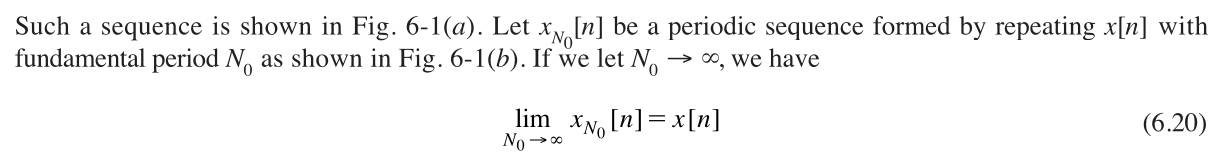
\includegraphics[width=\linewidth]{img/img02}
			\caption{Periodic sequence formed by periodic extension of $ x[n] $}
			\label{fig:img02}
		\end{figure}
	
		\item If we let $ N_0 \rightarrow \infty$, we have
		
		\begin{equation}\label{eq:01}
			\lim_{N_0 \rightarrow \infty} x_{N_0}[n] = x[n]
		\end{equation}
	
	\end{itemize}
\end{frame}

\begin{frame}{From Discrete Fourier Series to Fourier Transform:}
	\begin{itemize}
		\item The discrete Fourier series of $ x_N[n] $ is given by
		
		\begin{equation}\label{eq:02}
			x_{N_0}[n] = \sum\limits_{k=<N_0>} c_k e^{j k \Omega_0 n}\qquad \Omega_0 = \frac{2 \pi}{N_0}
		\end{equation}
		
		where
		
		\begin{equation}\label{eq:03}
			c_k = \frac{1}{N_0}\sum\limits_{n=<N_0>} x_{N_0}[n]e^{-j k \Omega_0 n}
		\end{equation}
		
	\end{itemize}
\end{frame}

\begin{frame}{From Discrete Fourier Series to Fourier Transform:}
	\begin{itemize}
		\item Since $ x_{N_0}[n] = x[n] $ for $ |n| \leq N_1 $ and also since $ x[n] = 0 $ outside this interval, Eq. \ref{eq:03} can be rewritten as
		
		\begin{equation}\label{eq:03}
			c_k = \frac{1}{N_0}\sum\limits_{n=<N_0>} x_{N_0}[n]e^{-j k \Omega_0 n}
		\end{equation}
	
	\end{itemize}
\end{frame}

\end{document}
